\documentclass[12pt]{article}
\usepackage[utf8]{inputenc}
\usepackage[russian]{babel}
\usepackage{array}
\usepackage{makecell}
\usepackage{amsmath}
\usepackage{amssymb}
\usepackage{tikz}
\usepackage{pgfplots}

\usepackage{graphicx}
\graphicspath{ {./images/}}

\usepackage{geometry}
\geometry{
    left = 1cm,
    right = 2cm,
    top = 2cm,
    bottom = 2cm,
    bindingoffset = 1cm
}

\pgfplotsset{compat=1.18}

\begin{document}
\begin{center}
    \hfill \break
    \hfill \break
    Санкт-Петербургский национальный исследовательский университет \\
    информационных технологий, механики и оптики \\
    \textbf{Учебный центр общей физики ФТФ} \\
    \vspace{12pt}
    \begin{tabular}[l]{m{0.2\textwidth} m{0.2\textwidth} m{0.4\textwidth}}
        \hline
        \textbf{Группа:} & Group & \textbf{К работе допущен:} \\
        \textbf{Студент:} & sltKaguya & \textbf{Работа выполнена:} \\
        \textbf{Преподаватель:} & Teacher & \textbf{Отчёт принят:}
    \end{tabular} \break
    \hfill \break
    \Large{\textbf{Рабочий протокол и отчёт по \\
    лабораторной работе №1.01}} \break
    
    \large{Исследование распределения случайной величины\\}\hfill
\end{center}

\begin{enumerate}
    \item Цель работы: \\
    Исследование распределения случайной величины.
    
    \item Задачи, решаемые при выполнении работы:
    \begin{enumerate}
        \item Провести многократные измерения определённого интервала времени.
        \item Построить гистограмму распределения результатов измерения.
        \item Вычислить среднее значение и дисперсию полученной выборки.
        \item Сравнить гистограмму с графиком функции Гаусса с такими же как и у экспериментального распределения средним значением и дисперсией.
    \end{enumerate} 

    \item Объект исследования: \\
    Случайная величина.

    \item Метод экспериментального исследования: \\
    Прямое измерение (времени).

    \item Рабочие формулы и исходные данные: \\
    $N$ -- полное количество измерений. \\
    $\langle t\rangle = \frac{1}{N}(t_1 + t_2 + \dots + t_N) = \frac{1}{N}\sum\limits_{i=1}^N t_i$ -- среднее арифметическое всех измерений. \\
    $\Delta N$ -- количество результатов, попавших в интервал $[t; t + \Delta t]$. \\
    $\sigma_N = \sqrt{\frac{1}{N-1} \sum\limits_{i=1}^N (t_i - \langle t\rangle_N)^2}$ -- выборочное среднеквадратичное отклонение. \\
    $\rho(t) = \frac{1}{\sigma\sqrt{2\pi}}\exp\left(-\frac{\left(t - \langle t\rangle\right)^2}{2\sigma^2}\right)$ -- функция Гаусса, описывает нормальное распределение. \\
    $\rho_{max} = \frac{1}{\sigma \sqrt{2 \pi}}$ -- максимальное значение плотности распределения. \\
    $\Delta\langle t\rangle = t_{\alpha, N}\cdot\sigma_{\langle t\rangle}$ -- расчёт доверительного интервала. \\
    $\alpha = 0.95$ -- доверительная вероятность. \\
    $t_{\alpha, N} = 2.0086$ -- коэффициент Стьюдента (табличный). \\
    $\sigma_{\langle t\rangle} = \sqrt{\frac{1}{N(N-1)}\sum\limits_{i=1}^N\left(t_i - \langle t\rangle_N\right)^2}$ -- среднеквадратичное отклонение среднего значения. \\
    $\Delta t = \sqrt{\theta_{\text{приб.}}^2 + \Delta^2 \langle t\rangle}$ -- расчёт абсолютной погрешности. \\
    $\delta = \frac{\Delta t}{\langle t\rangle}100\%$ -- расчёт относительной погрешности. \\
    $\left.\begin{array}{ll}
        t \in [\langle t\rangle - \sigma, \langle t\rangle + \sigma], & P_\sigma = 0.683 \\
        t \in [\langle t\rangle - 2\sigma, \langle t\rangle + 2\sigma], & P_\sigma = 0.954 \\
        t \in [\langle t\rangle - 3\sigma, \langle t\rangle + 3\sigma], & P_\sigma = 0.997
    \end{array}\right\}$ -- вероятность для номрального распределения в случае стандартных интервалов.

    \item Измерительные приборы: \\    
    \begin{tabular}{|m{0.07\linewidth}|m{0.18\linewidth}|m{0.17\linewidth}|m{0.2\linewidth}|m{0.18\linewidth}|}
        \hline
        № п/п & Наименование & Тип прибора & \makecell{Используемый\\ диапазон} & \makecell{Погрешность\\ прибора} \\
        \hline
        1 & Секундомер & Электронный & От 0 до 6 с & 0.01 с \\
        \hline
    \end{tabular}

    \item Схема установки:

    \item Результаты прямых измерений и их обработки: \\
    \begin{tabular}[l]{|m{0.2\textwidth}|m{0.2\textwidth}|m{0.2\textwidth}|m{0.2\textwidth}|}
    \hline
    № & $t_i$, с & $t_i - \langle t\rangle_N$, с & $\left(t_i - \langle t\rangle_N\right)^2, \text{ с}^2$\\
    \hline
    1 & 5.110 & 0.0112 & 0.00012544 \\
    \hline
    2 & 5.090 & -0.0088 & 0.00007744 \\
    \hline
    3 & 5.090 & -0.0088 & 0.00007744 \\
    \hline
    4 & 5.060 & -0.0388 & 0.00150544 \\
    \hline
    5 & 5.030 & -0.0688 & 0.00473344 \\
    \hline
    6 & 5.260 & 0.1612 & 0.02598544 \\
    \hline
    7 & 5.200 & 0.1012 & 0.01024144 \\
    \hline
    8 & 5.270 & 0.1712 & 0.02930944 \\
    \hline
    9 & 4.980 & -0.1188 & 0.01411344 \\
    \hline
    10 & 5.010 & -0.0888 & 0.00788544 \\
    \hline
    11 & 5.090 & -0.0088 & 0.00007744 \\
    \hline
    12 & 5.090 & -0.0088 & 0.00007744 \\
    \hline
    13 & 5.160 & 0.0612 & 0.00374544 \\
    \hline
    14 & 5.060 & -0.0388 & 0.00150544 \\
    \hline
    15 & 5.480 & 0.3812 & 0.14531344 \\
    \hline
    16 & 5.170 & 0.0712 & 0.00506944 \\
    \hline
    17 & 5.090 & -0.0088 & 0.00007744 \\
    \hline
    18 & 5.130 & 0.0312 & 0.00097344 \\
    \hline
    19 & 5.110 & 0.0112 & 0.00012544 \\
    \hline
    20 & 5.040 & -0.0588 & 0.00345744 \\
    \hline
    21 & 5.060 & -0.0388 & 0.00150544 \\
    \hline
    22 & 5.060 & -0.0388 & 0.00150544 \\
    \hline
    23 & 4.980 & -0.1188 & 0.01411344 \\
    \hline
    24 & 5.180 & 0.0812 & 0.00659344 \\
    \hline
    25 & 5.030 & -0.0688 & 0.00473344 \\
    \hline
    26 & 5.240 & 0.1412 & 0.01993744 \\
    \hline
    27 & 5.140 & 0.0412 & 0.00169744 \\
    \hline
    28 & 5.180 & 0.0812 & 0.00659344 \\
    \hline
    \end{tabular}

    \begin{tabular}[l]{|m{0.2\textwidth}|m{0.2\textwidth}|m{0.2\textwidth}|m{0.2\textwidth}|}
    \hline
    29 & 5.110 & 0.0112 & 0.00012544 \\
    \hline
    30 & 5.010 & -0.0888 & 0.00788544 \\
    \hline
    31 & 5.010 & -0.0888 & 0.00788544 \\
    \hline
    32 & 5.160 & 0.0612 & 0.00374544 \\
    \hline
    33 & 5.090 & -0.0088 & 0.00007744 \\
    \hline
    34 & 4.960 & -0.1388 & 0.01926544 \\
    \hline
    35 & 5.080 & -0.0188 & 0.00035344 \\
    \hline
    36 & 5.130 & 0.0312 & 0.00097344 \\
    \hline
    37 & 5.140 & 0.0412 & 0.00169744 \\
    \hline
    38 & 4.960 & -0.1388 & 0.01926544 \\
    \hline
    39 & 5.180 & 0.0812 & 0.00659344 \\
    \hline
    40 & 5.060 & -0.0388 & 0.00150544 \\
    \hline
    41 & 5.080 & -0.0188 & 0.00035344 \\
    \hline
    42 & 4.960 & -0.1388 & 0.01926544 \\
    \hline
    43 & 5.030 & -0.0688 & 0.00473344 \\
    \hline
    44 & 5.300 & 0.2012 & 0.04048144 \\
    \hline
    45 & 5.110 & 0.0112 & 0.00012544 \\
    \hline
    46 & 4.990 & -0.1088 & 0.01183744 \\
    \hline
    47 & 5.110 & 0.0112 & 0.00012544 \\
    \hline
    48 & 4.980 & -0.1188 & 0.01411344 \\
    \hline
    49 & 5.060 & -0.0388 & 0.00150544 \\
    \hline
    50 & 5.040 & -0.0588 & 0.00345744 \\
    \hline
    & $\langle t\rangle_N = 5.0988$ с & $\sum\limits_{i=1}^N t_i - \langle t\rangle_N = 0$ с & \makecell{$\sigma_N \approx 0.09861573$ \\$\rho_{max} \approx 4.04542237$} \\
    \hline
    \end{tabular}

    \item Расчёт результатов косвенных измерений: \\
    $t_{min} = 4.96, \ t_{max} = 5.48, \ \sqrt{N} \approx 7$ \\
    К промежутку $[t_{min}; t_{max}]$ длиной в 0.52 (с) были добавлены по 0.02 (с) с каждой стороны, таким образом промежуток $[4.94; 5.50]$ делится на 7 равных участков, $\Delta t = 0.08$ (с). \\
    \begin{tabular}[1]{|m{0.18\textwidth}|m{0.1\textwidth}|m{0.15\textwidth}|m{0.15\textwidth}|m{0.15\textwidth}|}
    \hline
    \makecell{Границы \\интервала} & $\Delta N$ & $\frac{\Delta N}{N\Delta t}, \text{ с}^{-1}$ & $t$, c & $\rho, \text{ c}^{-1}$ \\
    \hline
    \makecell{4.94 \\5.02} & 10 & 2.50 & 4.98 & 1.9581 \\
    \hline
    \makecell{5.02 \\5.10} & 19 & 4.75 & 5.06 & 3.7441 \\
    \hline
    \makecell{5.10 \\5.18} & 15 & 3.75 & 5.14 & 3.7073 \\
    \hline
    \makecell{5.18 \\5.26} & 3 & 0.75 & 5.22 & 1.9009 \\
    \hline
    \makecell{5.26 \\5.34} & 2 & 0.5 & 5.30 & 0.5047 \\
    \hline
    \makecell{5.34 \\5.42} & 0 & 0 & 5.38 & 0.0694 \\
    \hline
    \makecell{5.42 \\5.50} & 1 & 0.25 & 5.46 & 0.0049 \\
    \hline
    \end{tabular}

    Стандартные доверительные интервалы: \\
    \begin{tabular}[1]{|m{0.1\textwidth}|m{0.18\textwidth}|m{0.15\textwidth}|m{0.15\textwidth}|m{0.15\textwidth}|}
    \hline
    & \makecell{Интервал, с \\ от \qquad до} & $\Delta N$ & $\frac{\Delta N}{N}$ & $P$ \\
    \hline
    $\langle t\rangle \pm \sigma_N$ & 5.00 \qquad 5.20 & 38 & 0.76 & 0.683 \\
    \hline
    $\langle t\rangle \pm 2\sigma_N$ & 4.90 \qquad 5.30 & 49 & 0.98 & 0.954 \\
    \hline
    $\langle t\rangle \pm 3\sigma_N$ & 4.80 \qquad 5.39 & 50 & 1 & 0.997 \\
    \hline
    \end{tabular}
    \item Расчёт погрешностей измерения: \\
    $\sigma_{\langle t\rangle} = 0.0139$ \\
    Абсолютная погрешность: \\
    $\Delta\langle t\rangle = 0.198079555278$ \\
    $\Delta t = \sqrt{0.01^2 + 0.198079555278^2} \approx 0.1983$ (с). \\
    Относительная погрешность: \\
    $\delta_t \approx 3.890\%$.

    \item Графики: гистограмма и график плотности вероятности измеренного значения: \\
    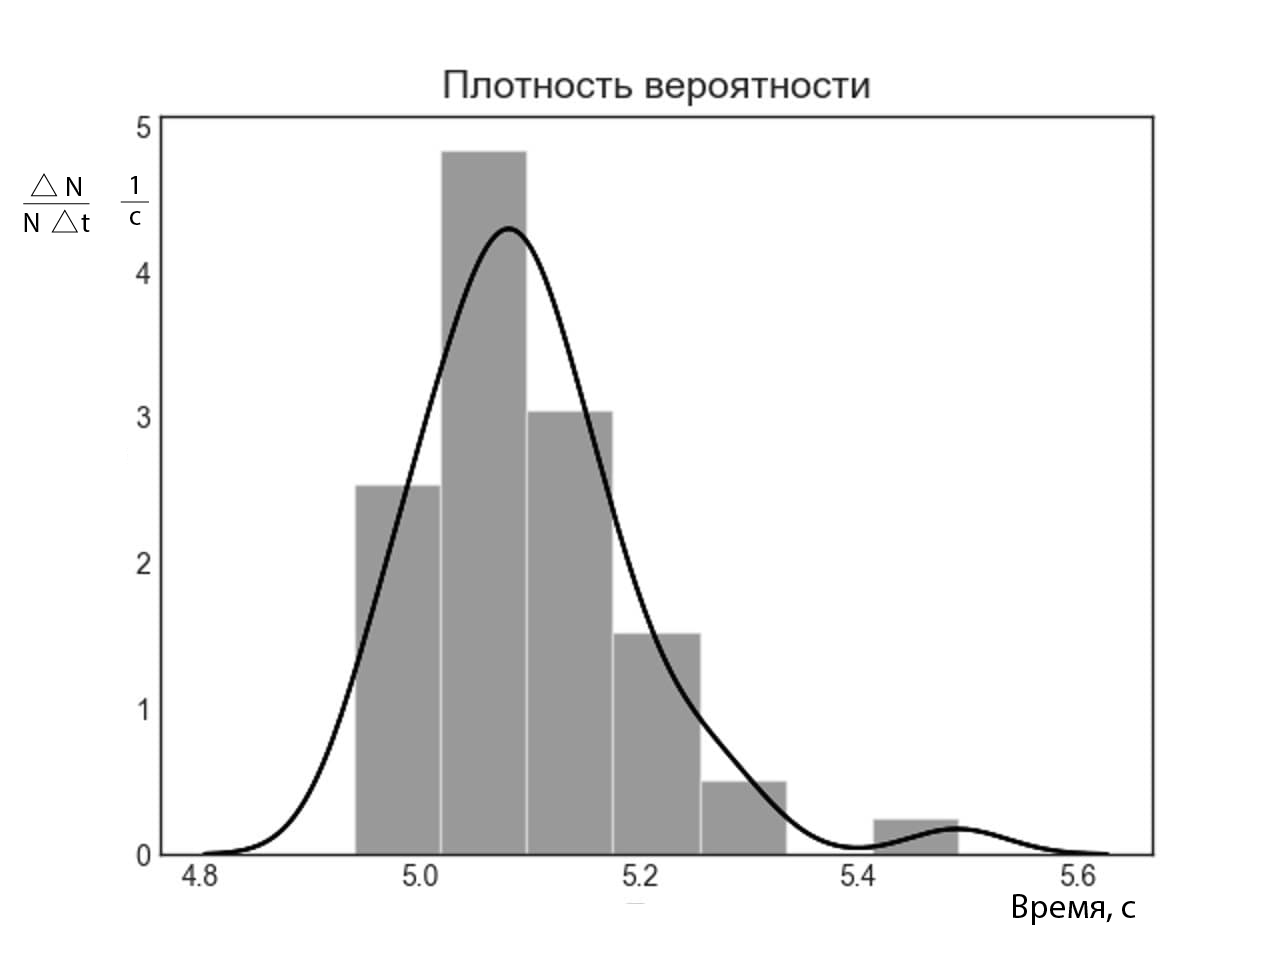
\includegraphics[scale=0.3]{gistogramm_2.png}

    \item Окончательные результаты: \\
    $t = \langle t\rangle + \Delta t = 5.0988 \pm 0.1981$ с. \\
    На основе 50 прямых измерений и ещё кучи косвенных была построена гистограмма распределения значений и график нормального распределения для данных значений.

    \item Выводы и анализы результатов работы: \\
    Был исселдован закон распределения случайной величины, построена гистограмма и функция Гаусса для сравнения. Гистограмма вполне соответствует графику
    
    \item Дополнительные задания:

    \item Выполнение дополнительных заданий:

    \item Замечания преподавателя:    
\end{enumerate}
\end{document}